\documentclass[11pt]{article}

\usepackage[margin=1in]{geometry}
\usepackage{amsmath, amssymb}
\usepackage{booktabs}
\usepackage{xcolor}
\usepackage{tikz}
\usetikzlibrary{arrows.meta, positioning, calc}
\usepackage{hyperref}

% Visible placeholder for unfinished steps -- delete every \todo before submitting.
\newcommand{\todo}[1]{\textcolor{red}{\textbf{[TODO: #1]}}}
\newcommand{\blank}{\underline{\hspace{1.5cm}}}
\newcommand{\indep}{\perp}

\title{CSE 5830: Probabilistic Graph Analysis \\ Homework 3}
\author{}
\date{Due 11:59PM, Wednesday 9/30/2026}

\begin{document}
\maketitle

Show all your work to get a full score.

% ============================================================
\section*{Problem 1: Noisy-AND (15 points)}

A Noisy-AND model (independence of the causal mechanisms when all $X$s are 1)
with binary random variables and leaky parameters
$(\lambda_0, \lambda_1, \dots, \lambda_K)$.

\subsection*{(a) Expression for $P(Y=0 \mid X_1, \dots, X_K)$ (10 points)}

\textbf{Setup / convention.}
Noisy-AND is the De Morgan dual of noisy-OR. In a deterministic AND gate, a
single input $X_i = 0$ is enough to force $Y = 0$, and $Y = 1$ happens in
only one way: every input equals 1.
\begin{center}
\begin{tabular}{cc|c}
  \toprule
  $X_1$ & $X_2$ & $Y = X_1 \land X_2$ \\
  \midrule
  0 & 0 & 0 \\
  0 & 1 & 0 \\
  1 & 0 & 0 \\
  1 & 1 & 1 \\
  \bottomrule
\end{tabular}
\end{center}
For each parent, introduce an independent mechanism variable $Z_i$, where
$Z_i = 1$ means ``$X_i$ forces $Y = 0$''. An input that is present can never
force an AND gate to 0, so
\[
  P(Z_i = 1 \mid X_i = 1) = 0, \qquad
  P(Z_i = 1 \mid X_i = 0) = \lambda_i .
\]
That is, $\lambda_i$ is the probability that an absent input ($X_i = 0$)
succeeds in forcing $Y = 0$. The leak $Z_0$ is always active, with
$P(Z_0 = 1) = \lambda_0$: the probability that $Y = 0$ even when every input
is 1. Then $Y = 1$ if and only if $Z_0 = Z_1 = \cdots = Z_K = 0$.

\textbf{Derivation.}
Since $Y = 1$ requires that no mechanism fires, and the mechanisms are
independent (independence of the causal mechanisms),
\[
  P(Y = 1 \mid X_1, \dots, X_K)
  = P(Z_0 = 0) \prod_{i=1}^{K} P(Z_i = 0 \mid X_i).
\]
Each factor is
\[
  P(Z_i = 0 \mid X_i) =
  \begin{cases}
    1, & X_i = 1, \\
    1 - \lambda_i, & X_i = 0,
  \end{cases}
\]
so parents with $X_i = 1$ contribute a factor of 1 and drop out. Hence
\[
  P(Y = 1 \mid X_1, \dots, X_K) = (1 - \lambda_0) \prod_{i \,:\, X_i = 0} (1 - \lambda_i),
\]
and taking the complement,
\[
  \boxed{\,P(Y = 0 \mid X_1, \dots, X_K)
  = 1 - (1 - \lambda_0) \prod_{i \,:\, X_i = 0} (1 - \lambda_i)\,}
\]

\textbf{Sanity check.} With no leak ($\lambda_0 = 0$) and $\lambda_i = 1$ for
all $i$: if every $X_i = 1$, the product is empty (equal to 1), so
$P(Y = 0) = 0$; if any $X_i = 0$, the product contains a factor $1 - 1 = 0$,
so $P(Y = 0) = 1$. This is exactly the deterministic AND gate.

\subsection*{(b) Numerical case (5 points)}

$K = 4$, \quad $\lambda_0 = 0,\ \lambda_1 = 0.9,\ \lambda_2 = 0.75,\
\lambda_3 = 0.8,\ \lambda_4 = 0.85$.

Only $X_2$ and $X_3$ are off, so only $\lambda_2$ and $\lambda_3$ enter the
product; $X_1 = X_4 = 1$ contribute factors of 1. With no leak,
$1 - \lambda_0 = 1$. Using the formula from (a):
\begin{align*}
  P(Y = 0 \mid X_1 = 1, X_2 = 0, X_3 = 0, X_4 = 1)
  &= 1 - (1 - \lambda_0)(1 - \lambda_2)(1 - \lambda_3) \\
  &= 1 - (1 - 0)(1 - 0.75)(1 - 0.8) \\
  &= 1 - (1)(0.25)(0.2) \\
  &= 1 - 0.05 \\
  &= \boxed{0.95}
\end{align*}

\textbf{Sanity check.} Two inputs are off, and each has a high chance
($0.75$ and $0.8$) of forcing $Y = 0$. So $Y = 1$ requires both of those
mechanisms to fail, which happens with probability only
$0.25 \times 0.2 = 0.05$. A value of $P(Y = 0)$ close to, but below, 1 is what
we expect.

% ============================================================
\section*{Problem 2: Factor product (15 points)}

Given factors:
\begin{center}
\begin{tabular}{cc|c}
  \toprule
  $X$ & $Y$ & $\phi_1(X,Y)$ \\
  \midrule
  1 & 1 & 0.8 \\
  1 & 2 & 0.5 \\
  2 & 1 & 0.5 \\
  2 & 2 & 0.6 \\
  \bottomrule
\end{tabular}
\qquad
\begin{tabular}{cc|c}
  \toprule
  $Y$ & $Z$ & $\phi_2(Y,Z)$ \\
  \midrule
  1 & 1 & 0.2 \\
  1 & 2 & 0.2 \\
  2 & 1 & 0.9 \\
  2 & 2 & 1.0 \\
  \bottomrule
\end{tabular}
\end{center}

\subsection*{(a) $\psi(X,Y,Z) = \phi_1(X,Y)\,\phi_2(Y,Z)$ (10 points)}

\begin{center}
\begin{tabular}{ccc|c|c}
  \toprule
  $X$ & $Y$ & $Z$ & $\phi_1(X,Y)\cdot\phi_2(Y,Z)$ & $\psi(X,Y,Z)$ \\
  \midrule
  1 & 1 & 1 & $0.8 \cdot 0.2$ & 0.16 \\
  1 & 1 & 2 & $0.8 \cdot 0.2$ & 0.16 \\
  1 & 2 & 1 & $0.5 \cdot 0.9$ & 0.45 \\
  1 & 2 & 2 & $0.5 \cdot 1.0$ & 0.5 \\
  2 & 1 & 1 & $0.5 \cdot 0.2$ & 0.1 \\
  2 & 1 & 2 & $0.5 \cdot 0.2$ & 0.1 \\
  2 & 2 & 1 & $0.6 \cdot 0.9$ & 0.54 \\
  2 & 2 & 2 & $0.6 \cdot 1.0$ & 0.6 \\
  \bottomrule
\end{tabular}
\end{center}

\subsection*{(b) $\psi(X,Z \mid Y=1)$ (5 points)}

This is a factor reduction to the context $Y = 1$: keep only the rows of
$\psi(X,Y,Z)$ from (a) with $Y = 1$ and drop the $Y$ column. Reduction alone
does not normalize, so the unnormalized values are shown first. To read
$\psi(X,Z \mid Y=1)$ as a conditional distribution, divide each entry by
their sum, $0.16 + 0.16 + 0.1 + 0.1 = 0.52$.

\begin{center}
\begin{tabular}{cc|c|c}
  \toprule
  $X$ & $Z$ & $\psi[Y=1]$ (reduced) & $\psi(X,Z \mid Y=1)$ (normalized) \\
  \midrule
  1 & 1 & 0.16 & $0.16/0.52 \approx 0.308$ \\
  1 & 2 & 0.16 & $0.16/0.52 \approx 0.308$ \\
  2 & 1 & 0.1  & $0.1/0.52 \approx 0.192$ \\
  2 & 2 & 0.1  & $0.1/0.52 \approx 0.192$ \\
  \midrule
  \multicolumn{2}{c|}{Sum} & 0.52 & 1 \\
  \bottomrule
\end{tabular}
\end{center}

% ============================================================
\section*{Problem 3: Pairwise Markov network (10 points)}

\[
  p(\mathbf{x}) \propto \phi(x_1,x_2)\,\phi(x_2,x_3)\,\phi(x_3,x_4)\,\phi(x_4,x_1)
\]

\subsection*{(a) Draw the network (2 points)}

\begin{center}
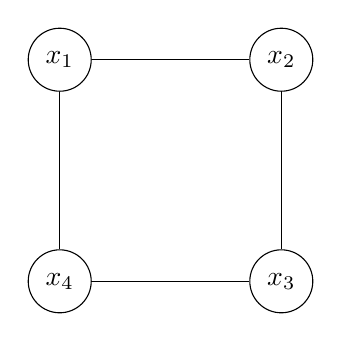
\begin{tikzpicture}[
    node distance=2cm,
    var/.style={circle, draw, minimum size=8mm}
  ]
  \node[var] (x1) {$x_1$};
  \node[var, right=of x1] (x2) {$x_2$};
  \node[var, below=of x2] (x3) {$x_3$};
  \node[var, below=of x1] (x4) {$x_4$};
  \draw (x1) -- (x2);
  \draw (x2) -- (x3);
  \draw (x3) -- (x4);
  \draw (x4) -- (x1);
\end{tikzpicture}
\end{center}

\subsection*{(b) Conditionals in terms of $\phi$ (8 points)}

\textbf{General method.} Write the conditional as a ratio of the joint to
its sum over the queried variable. The partition function $Z$ cancels, and
any factor that does not contain the queried variable takes the same value in
the numerator and in every term of the denominator, so it cancels too. Only
the factors touching the queried variable (that is, the edges to its two
neighbors) remain.

\paragraph{$p(x_1 \mid x_2, x_4)$.}
\[
  p(x_1 \mid x_2, x_4)
  = \frac{\tfrac1Z\,\phi(x_1,x_2)\,\phi(x_2,x_3)\,\phi(x_3,x_4)\,\phi(x_4,x_1)}
         {\sum_{x_1'}\tfrac1Z\,\phi(x_1',x_2)\,\phi(x_2,x_3)\,\phi(x_3,x_4)\,\phi(x_4,x_1')} .
\]
The factors $\phi(x_2,x_3)$ and $\phi(x_3,x_4)$ do not contain $x_1$, so they
cancel along with $\tfrac1Z$:
\[
  p(x_1 \mid x_2, x_4)
  = \frac{\phi(x_1,x_2)\,\phi(x_4,x_1)}{\sum_{x_1'}\phi(x_1',x_2)\,\phi(x_4,x_1')} .
\]

\paragraph{$p(x_2 \mid x_1, x_3)$.}
The factors containing $x_2$ are $\phi(x_1,x_2)$ and $\phi(x_2,x_3)$; the
factors $\phi(x_3,x_4)$ and $\phi(x_4,x_1)$ cancel.
\[
  p(x_2 \mid x_1, x_3)
  = \frac{\phi(x_1,x_2)\,\phi(x_2,x_3)}{\sum_{x_2'}\phi(x_1,x_2')\,\phi(x_2',x_3)} .
\]

\paragraph{$p(x_3 \mid x_2, x_4)$.}
The factors containing $x_3$ are $\phi(x_2,x_3)$ and $\phi(x_3,x_4)$; the
factors $\phi(x_1,x_2)$ and $\phi(x_4,x_1)$ cancel.
\[
  p(x_3 \mid x_2, x_4)
  = \frac{\phi(x_2,x_3)\,\phi(x_3,x_4)}{\sum_{x_3'}\phi(x_2,x_3')\,\phi(x_3',x_4)} .
\]

\paragraph{$p(x_4 \mid x_1, x_3)$.}
The factors containing $x_4$ are $\phi(x_3,x_4)$ and $\phi(x_4,x_1)$; the
factors $\phi(x_1,x_2)$ and $\phi(x_2,x_3)$ cancel.
\[
  p(x_4 \mid x_1, x_3)
  = \frac{\phi(x_3,x_4)\,\phi(x_4,x_1)}{\sum_{x_4'}\phi(x_3,x_4')\,\phi(x_4',x_1)} .
\]

\textbf{Observation.} Each conditional depends only on the variable's two
neighbors in the cycle. This is the local Markov property: a node is
independent of the rest of the network given its neighbors.

% ============================================================
\section*{Problem 4: Markov network structure (20 points)}

\begin{center}
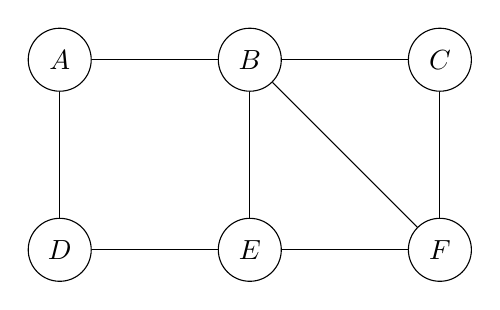
\begin{tikzpicture}[
    node distance=1.6cm,
    var/.style={circle, draw, minimum size=8mm}
  ]
  \node[var] (A) {$A$};
  \node[var, right=of A] (B) {$B$};
  \node[var, right=of B] (C) {$C$};
  \node[var, below=of A] (D) {$D$};
  \node[var, below=of B] (E) {$E$};
  \node[var, below=of C] (F) {$F$};
  \draw (A) -- (B);
  \draw (B) -- (C);
  \draw (A) -- (D);
  \draw (B) -- (E);
  \draw (C) -- (F);
  \draw (D) -- (E);
  \draw (E) -- (F);
  \draw (B) -- (F);
\end{tikzpicture}
\end{center}

\subsection*{(a) All factors that factorize over the graph (6 points)}

\textbf{Edges:} $A$--$B$, $A$--$D$, $B$--$C$, $B$--$E$, $B$--$F$, $C$--$F$,
$D$--$E$, $E$--$F$ \quad (8 edges).

\textbf{Cliques} (every pair of nodes in the set must be joined by an edge):
\begin{itemize}
  \item Single nodes: $\{A\}, \{B\}, \{C\}, \{D\}, \{E\}, \{F\}$.
  \item Edges: the 8 edges listed above.
  \item Triangles: $\{B,E,F\}$ (edges $B$--$E$, $E$--$F$, $B$--$F$) and
        $\{B,C,F\}$ (edges $B$--$C$, $C$--$F$, $B$--$F$).
  \item No 4-cliques: e.g.\ $\{A,B,D,E\}$ is missing $A$--$E$ and $B$--$D$,
        and $\{B,C,E,F\}$ is missing $C$--$E$.
\end{itemize}

\textbf{Maximal cliques:} the two triangles $\{B,E,F\}$ and $\{B,C,F\}$, plus
the edges not contained in either triangle: $\{A,B\}$, $\{A,D\}$, $\{D,E\}$.

A distribution factorizes over this graph if it can be written as a product
of factors over its maximal cliques (factors over smaller cliques can be
absorbed into these):
\[
  P(A,B,C,D,E,F) = \frac{1}{Z}\,
  \phi_1(A,B)\,\phi_2(A,D)\,\phi_3(D,E)\,\phi_4(B,E,F)\,\phi_5(B,C,F),
\]
\[
  Z = \sum_{a,b,c,d,e,f}
  \phi_1(a,b)\,\phi_2(a,d)\,\phi_3(d,e)\,\phi_4(b,e,f)\,\phi_5(b,c,f).
\]

\subsection*{(b) Gibbs distribution as a pairwise MN (6 points)}

A pairwise Markov network has one factor per edge (and optionally one
per node), even for edges that lie inside a triangle. Using the 8 edges:
\[
  P(A,B,C,D,E,F) = \frac{1}{Z}\,
  \phi(A,B)\,\phi(A,D)\,\phi(B,C)\,\phi(B,E)\,\phi(B,F)\,\phi(C,F)\,\phi(D,E)\,\phi(E,F),
\]
\[
  Z = \sum_{a,b,c,d,e,f}
  \phi(a,b)\,\phi(a,d)\,\phi(b,c)\,\phi(b,e)\,\phi(b,f)\,\phi(c,f)\,\phi(d,e)\,\phi(e,f).
\]
Unlike in (a), the triangles $\{B,E,F\}$ and $\{B,C,F\}$ are not given their
own 3-variable factors; each is represented only through its three
pairwise edge factors.

\subsection*{(c) Local Markov independencies (6 points)}

In a Markov network, each node is independent of all other nodes given its
neighbors (its Markov blanket):
$X \indep \bigl(\mathcal{X} \setminus (\{X\} \cup \mathrm{MB}(X))\bigr) \mid \mathrm{MB}(X)$.

\begin{center}
\begin{tabular}{c|c|l}
  \toprule
  Node & Neighbors (Markov blanket) & Local independence \\
  \midrule
  $A$ & $\{B, D\}$       & $A \indep \{C, E, F\} \mid \{B, D\}$ \\
  $B$ & $\{A, C, E, F\}$ & $B \indep \{D\} \mid \{A, C, E, F\}$ \\
  $C$ & $\{B, F\}$       & $C \indep \{A, D, E\} \mid \{B, F\}$ \\
  $D$ & $\{A, E\}$       & $D \indep \{B, C, F\} \mid \{A, E\}$ \\
  $E$ & $\{B, D, F\}$    & $E \indep \{A, C\} \mid \{B, D, F\}$ \\
  $F$ & $\{B, C, E\}$    & $F \indep \{A, D\} \mid \{B, C, E\}$ \\
  \bottomrule
\end{tabular}
\end{center}

\subsection*{(d) Is $A \indep F \mid \{D, C\}$? (2 points)}

\textbf{No.} In a Markov network, $A \indep F \mid \{D, C\}$ holds only if
every path from $A$ to $F$ passes through an observed node in $\{D, C\}$
(separation). The path
\[
  A - B - F
\]
uses only the unobserved node $B$, so it is active. ($A - B - E - F$ is
another active path.) Hence $A$ and $F$ are not separated by $\{D, C\}$,
and they are not independent given $D$ and $C$. Observing $D$ and $C$ blocks
only the paths $A - D - E - F$ and $A - B - C - F$, not the route through
$B$.

% ============================================================
\section*{Problem 5: Tree-structured CPD (10 points)}

Leaves list $(P(e^0), P(e^1))$.

\begin{center}
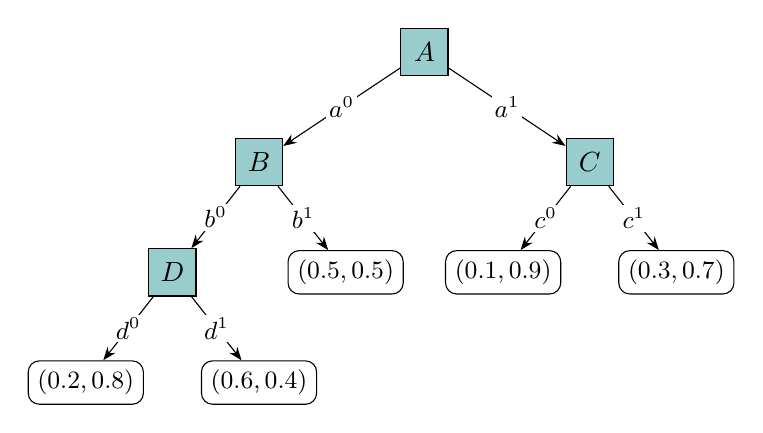
\begin{tikzpicture}[
    level distance=1.4cm,
    level 1/.style={sibling distance=4.2cm},
    level 2/.style={sibling distance=2.2cm},
    inner/.style={rectangle, draw, fill=teal!40, minimum size=6mm},
    leaf/.style={rectangle, draw, rounded corners, font=\small},
    edge from parent/.style={draw, -{Stealth}},
    lab/.style={font=\small, midway, fill=white, inner sep=1pt}
  ]
  \node[inner] {$A$}
    child { node[inner] {$B$}
      child { node[inner] {$D$}
        child { node[leaf] {$(0.2, 0.8)$} edge from parent node[lab] {$d^0$} }
        child { node[leaf] {$(0.6, 0.4)$} edge from parent node[lab] {$d^1$} }
        edge from parent node[lab] {$b^0$} }
      child { node[leaf] {$(0.5, 0.5)$} edge from parent node[lab] {$b^1$} }
      edge from parent node[lab] {$a^0$} }
    child { node[inner] {$C$}
      child { node[leaf] {$(0.1, 0.9)$} edge from parent node[lab] {$c^0$} }
      child { node[leaf] {$(0.3, 0.7)$} edge from parent node[lab] {$c^1$} }
      edge from parent node[lab] {$a^1$} };
\end{tikzpicture}
\end{center}

To read the tree CPD, start at the root and follow the branch matching
each observed value until a leaf is reached. Variables not on that path do
not affect the result.

\subsection*{(a) $P(E=e^0 \mid a^0, b^1, c^1, d^1)$}
Path: $A \xrightarrow{a^0} B \xrightarrow{b^1} (0.5, 0.5)$. The values of
$C$ and $D$ are irrelevant in this context.
\[
  P(E = e^0 \mid a^0, b^1, c^1, d^1) = \boxed{0.5}
\]

\subsection*{(b) $P(E=e^1 \mid a^1, b^1, c^1, d^1)$}
Path: $A \xrightarrow{a^1} C \xrightarrow{c^1} (0.3, 0.7)$. The values of
$B$ and $D$ are irrelevant in this context.
\[
  P(E = e^1 \mid a^1, b^1, c^1, d^1) = \boxed{0.7}
\]

\subsection*{(c) $P(E=e^1 \mid a^0, b^0, c^0, d^0)$}
Path: $A \xrightarrow{a^0} B \xrightarrow{b^0} D \xrightarrow{d^0} (0.2, 0.8)$.
The value of $C$ is irrelevant in this context.
\[
  P(E = e^1 \mid a^0, b^0, c^0, d^0) = \boxed{0.8}
\]

\subsection*{(d) Is $E \indep_c B \mid a^0$?}
\textbf{No.} In the context $a^0$, the tree splits on $B$, and the two
branches lead to different distributions over $E$:
\[
  P(E \mid a^0, b^1) = (0.5, 0.5),
  \qquad
  P(E \mid a^0, b^0, d^0) = (0.2, 0.8),
  \qquad
  P(E \mid a^0, b^0, d^1) = (0.6, 0.4).
\]
For example, with $d^0$, changing $B$ from $b^1$ to $b^0$ changes
$P(e^1)$ from $0.5$ to $0.8$. So $P(E \mid a^0, B, \cdot)$ depends on $B$,
and $E$ is not context-specifically independent of $B$ given $a^0$.

\subsection*{(e) Is $E \indep_c C \mid d^1$?}
\textbf{No.} The context $d^1$ fixes only $D$, and $D$ appears only in the
$a^0, b^0$ subtree. It does not affect the $a^1$ branch, where the tree
splits on $C$:
\[
  P(E \mid a^1, c^0, d^1) = (0.1, 0.9),
  \qquad
  P(E \mid a^1, c^1, d^1) = (0.3, 0.7).
\]
So with $A = a^1$, changing $C$ changes the distribution of $E$ even when
$d^1$ is fixed. (Under $a^0$, $C$ is irrelevant, but context-specific
independence must hold for every value of the remaining variables, and it
fails when $A = a^1$.) Hence $E$ is not context-specifically independent of
$C$ given $d^1$.


\subsection*{Use of Ai}
In this assignment, I used Ai to help me understand the assignment give me hints for each question as well as helping whenever I got stuck in a question. Also used AI to write and debug my tex code. However, I solved all the question of the assignment on my own.
\end{document}
